\documentclass[journal]{IEEEtran}
\usepackage{graphicx}
\usepackage{booktabs}
\usepackage{amsmath}
\usepackage{amssymb}
\usepackage{algorithm}
\usepackage{algorithmic}
\usepackage{url}
\usepackage[table]{xcolor}
\definecolor{darkyellow}{rgb}{0.8, 0.6, 0.0}
\usepackage{caption}
\usepackage[margin=1in]{geometry}
\usepackage[T1]{fontenc}
\usepackage[utf8]{inputenc}
% \usepackage[hidelinks]{hyperref}
\usepackage{subcaption}
\usepackage{hyperref}
\hypersetup{
    colorlinks=true,
    linkcolor=blue,
    citecolor=green!95!black, % For scientific citations
    filecolor=magenta,      
    urlcolor=blue!80!black,
    pdftitle={RT-FedMTL: A Real-Time Federated Multi-Task Learning Framework with Small Language Models for Natural Language Understanding Tasks},
    pdfpagemode=FullScreen,
}
\newcommand{\valuelink}[2]{\begingroup\hypersetup{linkcolor=teal}\hyperlink{#1}{#2}\endgroup}
\let\oldeqref\eqref
\renewcommand{\eqref}[1]{\begingroup\hypersetup{linkcolor=violet}\oldeqref{#1}\endgroup}

\begin{document}

\title{RT-FedMTL: A Novel Real-Time Federated Multi-Task Learning Framework with Small Language Models for Natural Language Understanding Tasks}

\author{Quang-Vinh~Pham~and~Quang-Hung~Le
\thanks{Quang-Vinh~Pham is with the Department of Data Science, TMA Tech Group, Gia Lai, Vietnam (e-mail: pqvinh@tma.com.vn).}%
\thanks{Quang-Hung~Le is with the Department of Information Technology, Quy Nhon University, Vietnam (e-mail: lequanghung@qnu.edu.vn).\\
*~Corresponding author: Quang-Hung Le (lequanghung@qnu.edu.vn).\\
*~This research is conducted within the framework of science and technology projects at institutional level of Quy Nhon University, Vietnam under the project code T2026.923.07.}}

% The paper headers
\markboth{JOURNAL OF COMMUNICATIONS SOFTWARE AND SYSTEMS, VOL.~XX, NO.~X, MARCH~2026}
{Pham \MakeLowercase{\textit{et al.}}: RT-FedMTL: A Real-Time Federated Multi-Task Learning Framework}

\maketitle

\begin{abstract}
%1. State the problem
%2. Say why it’s an interesting problem
%3. Say what your solution achieves
%4. Say what follows from your solution

Natural language understanding is a crucial component in intelligent systems such as social media monitoring, conversational agents, and information retrieval. Deploying these systems in real application scenarios requires not only accurate but also efficient, privacy-preserving, and capable of handling multiple tasks simultaneously. Centralized training of large language models based approaches raises significant challenges in terms of data privacy, communication overhead, and inference latency. This paper proposes RT-FedMTL, a novel real-time federated multi-task learning framework with small language models for efficient and privacy-preserving natural language understanding. Particularly, our framework unifies federated learning and multi-task learning to enable collaborative training across distributed clients while preserving data locality and leveraging shared representations across tasks. We utilize WebSocket protocols and small language models tuning to reduce the feedback loop and provide near-instantaneous global updates. Extensive experiments conducted on five small language model architectures with respect to three standard natural language understanding tasks to get the best trade-off between performance and resource usage. A significant result demonstrates RT-FedMTL can drastically minimize per-client GPU memory requirements (up to 74-92\%) versus centralized multi-task learning baselines, while keeping performance for multiple benchmarks. The source code is available at: \url{https://github.com/vinh1988/RT-FedMTL.git}.
\end{abstract}

\begin{IEEEkeywords}
Federated Learning, Multi-Task Learning, Federated Multi-Task Learning,
Small Language Models, Natural Language Understanding.
\end{IEEEkeywords}

\IEEEpeerreviewmaketitle

\section{Introduction} \label{sec:introduction}
% NLU, applications: challenges and concerns
Natural language understanding (NLU) is a core module in advanced artificial intelligence language processing systems such as sentiment analysis \cite{socher2013recursive} for customer feedback, intent classification \cite{wang2018glue} for conversational agents, semantic similarity \cite{cer2017semeval} for information retrieval, and so on. According to the modern approach, these sytems have achieved impressive capabilities by leveraging large language models \cite{devlin2019bert}. However, they often require centralized training and deployment, which poses challenges related to data privacy, computational cost, and inference latency.

% SLMs: advantages, challenges and concerns
Consequently, recent research has shifted towards small language models (SLMs) \cite{sanh2019distilbert, turc2019well, wang2020minilm} due to their low inference latency and cost-effectiveness. These models are well-suited to resource-constrained environments, addressing the challenges of large language models \cite{li2020federated}. Nevertheless, SLMs are often limited in capacity, making it difficult to maintain high performance across a variety of NLU tasks.

%MTL: advantages, challenges and concerns
At the same time, multi-task learning (MTL) \cite{ruder2017overview, caruana1997multitask} has been widely adopted as an effective paradigm to solve multiple tasks simultaneously. This approach of leveraging useful information from related tasks can lead to better learning performance \cite{wang2018glue, yu2020gradient}. Despite its advantages, most existing multi-tasking learning methods typically require centralized training data, which is impractical in privacy-sensitive situations where data is distributed across multiple clients.

% FL: advantages, challenges and concerns
With the growing availability of sensitive textual data, strict privacy regulations such as the GDPR \cite{european2016regulation} have raised concerns about centralizing user data in conventional machine learning pipelines. These challenges have motivated the development of federated learning (FL), a distributed paradigm that enables model training across clients without transferring raw data to a central server, thereby preserving privacy while supporting large-scale learning \cite{mcmahan2017communication, yang2019federated}. 
However, current FL pipelines mainly depend on batch synchronization where clients execute multiple local steps and will execute the sync periodically \cite{mcmahan2017communication, li2020federated_prox}. This design is effective for static datasets but less so for streaming and dynamic environments where language patterns as well as subjects and user intent change with frequency. 

% Our proposal
To address the aforementioned challenges and concerns, this paper proposes RT-FedMTL, a novel real-time federated MTL framework with SLMs for NLU tasks. Particularly, our framework integrates FL and MTL to enable collaborative training across distributed clients while preserving data locality and leveraging shared representations across tasks. To the best of our knowledge, this is the first work to explore the use of WebSocket protocols and SLMs tuning to reduce the feedback loop and provide near-instantaneous global updates for a NLU-based federated MTL system. Our key contributions are
summarized as follows:
\begin{enumerate}
    \item We propose RT-FedMTL, a novel real-time federated framework of MTL and SLMs to harness cross-task knowledge transfer without causing a large amount of resources to be consumed on devices.
    \item We assess five SLM architectures (DistilBERT \cite{sanh2019distilbert}, BERT-Medium \cite{turc2019well}, BERT-Mini \cite{turc2019well}, MiniLM \cite{wang2020minilm}, and TinyBERT \cite{jiao2019tinybert}) with respect to three standard NLU tasks (sentiment analysis, paraphrase detection, and semantic similarity), to get the best trade-off between performance and resource usage.
    \item We investigate the effects of non-IID and task heterogeneity on convergence speed and task accuracy in real-time domain.
    \item We show RT-FedMTL can drastically minimize per-client GPU memory requirements (up to 74-93\%) versus centralized MTL baselines, while keeping performance for multiple benchmarks (GLUE suite).
\end{enumerate}

The remainder of the paper is organised as follows. Section~\ref{sec:problem_definition} defines the formal problem of RT-FedMTL and Section~\ref{sec:proposed_method} presents the proposed framework. Section~\ref{sec:experiments} describes the experimental setup and results analysis. The relevant work is briefly reviewed in Section~\ref{sec:related_work}. 
Finally, Section~\ref{sec:conclusion} concludes and outlines future work.

\section{Problem Formulation}  
\label{sec:problem_definition}  
This section introduces the RT-FedMTL environment for NLU. We define the formal mathematical structure for distributed multi-task optimization work, tackle the issues of data and system heterogeneity, and set the global goal for training collaboration models across private edge clients.

\subsection{System Setup}  
We model a NLU-based RT-FedMTL system in which training is carried out across communication rounds $t=1,2,\dots$ \cite{mcmahan2017communication,smith2017federated,chen2024fedbone}. In each round, a subset of clients is chosen, local updates are made to private data streams, and parameters are returned to a central server for aggregation. As opposed to offline FL, the client data distributions can vary over time. Hence, both local goals and optimum parameters are time-dependent. Let $\mathcal{C}=\{1,\dots,C\}$ represent the set of clients and $\mathcal{K}=\{1,\dots,K\}$ represent the set of NLU tasks. Each client $c\in\mathcal{C}$ is assigned to only one main task $\tau(c)\in\mathcal{K}$ (or a small subset of tasks), where new samples are added to the local stream perpetually. The goal is to learn a federated model with cross-task transfer quality but task-level specialization in the absence of IID and time-varying data.

\subsection{Learning Objective}  
Heterogeneity comes in two forms:  
\begin{itemize}  
\item Heterogeneity of data: the local distributions will differ across clients $c_i,c_j$ (i.e. $P_{c_i}(x,y)\neq P_{c_j}(x,y)$) (label skew, domain shift, vocabulary differences).  
\item Task heterogeneity: clients might optimize different losses according to $\tau(c)$, which will produce diverging gradients across tasks.  
\end{itemize}  
In addition, systems remain heterogeneous, stale updates are propagated by client availability and update frequency. Therefore, the optimization problem must include partial participation and nonuniform local progress. Let $\ell_{\tau(c)}(\theta_e,\theta_{\tau(c)};\xi)$ be the loss cost for the specific sample $\xi\in\mathcal{D}_c^t$. The universal goal at stage $t$ is  
\begin{equation}  \label{eq:universal_goal}
\begin{aligned}  
\min_{\theta_e,\{\theta_k\}} \,F_t(\Theta)  
&= \sum_{c=1}^{C} p_c^t \, \mathbb{E}_{\xi\sim\mathcal{D}_c^t}  
\big[\ell_{\tau(c)}(\theta_e,\theta_{\tau(c)};\xi)\big] \\  
&\quad + \lambda \, \Omega(\{\theta_k\}),  
\end{aligned}  
\end{equation}  
where $p_c^t$ denote the weight of the aggregated model (i.e., the weight per unit local sample), $\Omega$ is a regularizer to enhance the cross-task learning stability and $\lambda\ge0$ moderates the sharing-specialization trade-off. After local updates, the server also aggregates common encoder parameters through weighted averaging,  
\begin{equation}  \label{eq:encoder_aggregation}
\theta_e^{t+1} = \sum_{c\in\mathcal{C}_t} \alpha_c^t \, \theta_{e,c}^{t+1},  
\end{equation}  
and updates custom task-specific parameters, following task-wise aggregation,  
\begin{equation}  \label{eq:head_aggregation}
\theta_k^{t+1} = \sum_{c \in\mathcal{C}_t: \, \tau(c)=k} \beta_c^t \, \theta_{k,c}^{t+1}.  
\end{equation}  
In $\mathcal{C}_t$ the client subset participates at round $t$ and $\alpha_c^t,\beta_c^t$ can be viewed as normalized aggregation coefficients \cite{mcmahan2017communication,smith2017federated,zhou2025multi}. By working towards privacy and heterogeneity requirements, RT-FedMTL is captured as the architecture in real-time, jointly maximizing the optimal use of shared representations and task-specific parameters \eqref{eq:encoder_aggregation}, \eqref{eq:head_aggregation}.
\section{Proposed Framework}
\label{sec:proposed_method}

\begin{figure*}[t]
    \centering
    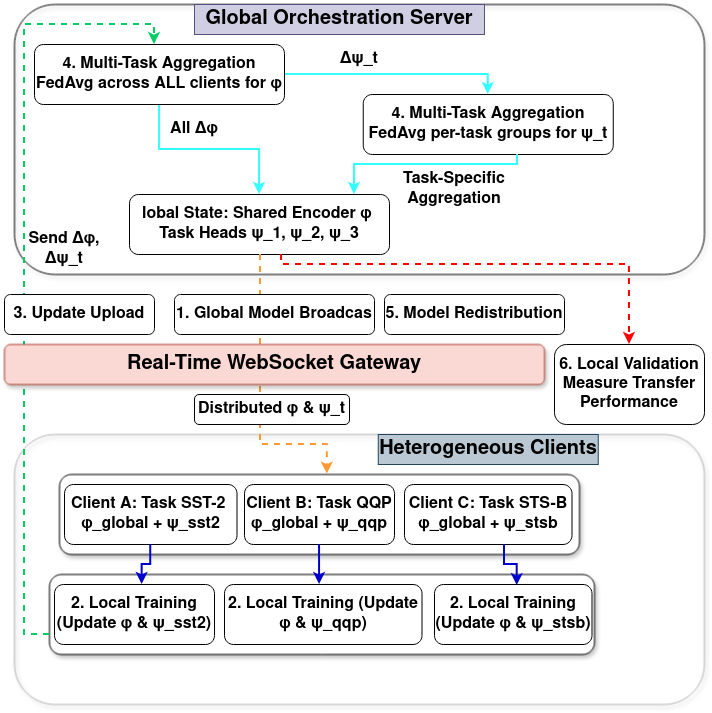
\includegraphics[width=0.85\textwidth]{plots/FL_MTL_FRAME_WORK.png}
    \caption{Architecture of the developed framework for real-time federated MTL.}
    \label{fig:framework_pipeline}
\end{figure*}

The proposed RT-FedMTL simultaneously addresses the challenges of balancing privacy-preserving NLU and resource-constrained edge computing. We introduce a modular federated-based architecture tailored for real-time asynchronous synchronization across WebSockets, multi-task learning (leveraging common linguistic representations with task-specific specialization), and parameter-efficient SLMs to reduce the computational and communication footprint on edge devices.

\subsection{System Overview}
As illustrated in Fig.~\ref{fig:framework_pipeline}, a high level orchestration server, and several heterogeneous client nodes form the basis of the architecture. A parameter server maintains a global state at the center and controls the model aggregation logic. The communications depend on low-latency WebSockets for a bidirectional exchange of model updates, and aggregated parameters.


Federated components and privacy constraints of a system are built on:
\begin{itemize}
    \item Global server $\mathcal{S}$: orchestrates client sampling, model broadcast, and aggregation.
    \item Distributed clients $\mathcal{C}$: edge devices/silos to store the raw text.
    \item Functional modules ($f_e, h_k$): the shared backbone and task-specific heads parameterized by $\theta_e, \theta_k$ (see Fig.~\ref{fig:framework_pipeline}).
    \item Local datasets $\mathcal{D}_c^t$: private data streams for the client $c$ at round $t$.
\end{itemize}

For the sake of privacy, samples are never uploaded. Each of these clients sends only model updates (or compressed adapter and head updates) and acts as host-side aggregation \cite{mcmahan2017communication,elbakary2025mira}. This is in line with the traditional federated privacy model in which data locality is retained and collaborative training is advocated in the field.

\subsection{Backbone of Small Language Model (SLMs)} This approach enables special SLMs for ensuring an optimal computational efficiency with high language understanding. We use architectures such as DistilBERT \cite{sanh2019distilbert}, BERT-Medium \cite{turc2019well}, MiniLM \cite{wang2020minilm} for resource-constrained environments. The SLM backbone consists of several integral stages:

\subsubsection{Tokenizer and Embedding Layer} Outputs are inputted and processed by input text subword tokenizer that converts raw strings into a series of tokens. The generated tokens map to a high-dimensional vector space by means of a learned embedding layer. To model sequence structures without the overhead of recurrences, we add learnable position embeddings at the level of the token embeddings providing the machine with necessary context about the order of the tokens.

\subsubsection{Low-Cost Transformer Encoder} The central element is a lightweight transformer encoder. These models consist of fewer layers and smaller hidden dimensionality than traditional BERT-base architectures \cite{devlin2019bert}. Each layer utilizes multi-head self-attention for long-range dependencies and the feed-forward network for feature transformation. This streamlined way significantly reduces parameter number and computational load, thus allowing for fast inference and training on edge devices.

\subsubsection{Shared Representation} The encoder generates a dense vector, represented as a shared representation $f_e(x; \theta_e)$. This captures the basic semantically and syntactically fundamental information in the input. In our multi-task framework, with the backbone shared across all tasks the model learns universal linguistic patterns while task specific heads focus on unique output. This federated learning-based collaborative tuning guarantees strong generalization across heterogeneous client data.

\subsection{Multi-Task Learning Strategy}
We adopt a hybrid approach of sharing the parameters. Throughout the tasks that all share linguistic representation, the lower (encoder) layers of the transformer remains unchanged. On the other hand, top layers are task-centric classification or regression heads respectively. We thus maintain an adaptive loss weighting mechanism to minimize negative transfer:
\begin{equation} \label{eq:total_multi_task_loss}
    \mathcal{L}_{total} = \sum_{j=1}^{K} w_j \mathcal{L}_j
\end{equation}
where $w_j$ are task weights dynamically tuned for each task $j$ based on the convergence rate. This formulation ensures that the local update step in Algorithm~\ref{alg:rt_fedmtl} minimizes the regularized objective function defined in Eq. \eqref{eq:universal_goal}.

We define the parameters
\begin{equation} \label{eq:parameter_set}
    \Theta = \{\theta_e, \{\theta_k\}_{k=1}^{K}\},
\end{equation}
where $\theta_e$ parameterizes the SLM encoder $f_e$ and $\theta_k$ parameterizes the task head $h_k$ for task $k$ \cite{chen2024fedbone,zhou2025multi}. Prediction for input $x$ in task $k$ is given by:
\begin{equation} \label{eq:prediction_head}
    \hat{y} = h_k\big(f_e(x;\theta_e);\theta_k\big),
\end{equation}
where $f_e(\cdot)$ and $h_k(\cdot)$ represent the components optimized in Algorithm~\ref{alg:rt_fedmtl} to maximize sharing while preserving task-specificity.

\subsection{Federated Optimization and Real-Time Adaptation}
The federated optimization process is described in Algorithm~\ref{alg:rt_fedmtl}. This system enables real-time adaptation by dynamically synchronizing updates on request via WebSockets. Using a task-aware version of FedAvg \cite{mcmahan2017communication}, the server aggregates updates and normalizes noise from heterogeneous sources (non-IID). Most recent work in adaptive federated optimization \cite{reddi2020adaptive} suggests incorporating momentum and adaptive learning rates will add an even greater level of stability.

\begin{algorithm}
\caption{RT-FedMTL: Real-time federated MTL}
\label{alg:rt_fedmtl}
\begin{algorithmic}[1]
\STATE Server Initialize: Shared encoder $\theta_{e,0}$, task heads $\{\theta_{j,0}\}_{j=1}^K$
\FOR{each round $t = 1, 2, \dots$}
    \STATE Server broadcasts $\theta_{e,t}, \theta_{Task(c),t}$ (for $f_e, h_k$) to clients $c \in \mathcal{C}_t$
    \FOR{each client $c \in \mathcal{C}_t$ in parallel}
        \STATE Local training: $\{\theta_{e,c}^{t+1}, \theta_{Task(c),c}^{t+1}\} \leftarrow \text{LocalUpdate}(\mathcal{D}_c, f_e, h_k, \theta_{e,t}, \theta_{Task(c),t})$ \COMMENT{Optimize $h_k(f_e(\cdot))$}
        \STATE Updates $\{\theta_{e,c}^{t+1}, \theta_{Task(c),c}^{t+1}\}$ via WebSockets to Server
    \ENDFOR
    \STATE Encoder Aggregation:
    \STATE \quad $\theta_{e,t+1} \leftarrow \sum_{c\in\mathcal{C}_t} \alpha_c^t \theta_{e,c}^{t+1}$ \COMMENT{Aggregate shared backbone $f_e$}
    \FOR{each task $k \in \{1,\dots,K\}$ in parallel}
        \STATE $\theta_{k,t+1} \leftarrow \sum_{c \in\mathcal{C}_t: \, \tau(c)=k} \beta_c^t \theta_{k,c}^{t+1}$ \COMMENT{Aggregate specialized head $h_k$}
    \ENDFOR
    \STATE Server assigns $\{\theta_{e,t+1}, \theta_{Task(c),t+1}\}$ for Local Validation
\ENDFOR
\end{algorithmic}
\end{algorithm}

\subsection{Communication-Efficient Fine-Tuning}
To further reduce resource usage in edge devices, we perform low-rank adaptation (LoRA) \cite{hu2022lora}. This ranges from updating in local $B$, where instead of updating the full weight matrices $W \in \mathbb{R}^{d \times d}$, we optimize the low rank decomposition matrices $A$ and $B$, where:
\begin{equation} \label{eq:lora_decomposition}
    W' = W + \Delta W = W + BA.
\end{equation}
$A \in \mathbb{R}^{r \times d}$ and $B \in \mathbb{R}^{d \times r}$ with rank $r \ll d$. When performing big updates, only the matrices $A$ and $B$ are sent, minimizing communication volume up to 99\%.
\section{EXPERIMENTS}
\label{sec:experiments}
In this section, the proposed RT-FedMTL framework is examined in terms of five thematic dimensions: overall baseline comparisons, the impact of MTL, paradigm performance gaps, real-time suitability, and communication efficiency.  
\subsection{Experimental Setup}  
\subsubsection{Datasets and Tasks}  
This evaluation combines three core NLU benchmarks that represent different NLU problems from within the GLUE benchmark \cite{wang2018glue}. SST-2 \cite{socher2013recursive} is a binary classification task (66,477 training, 872 validation, 1,821 test samples) for detecting sentiment polarity. The performance is determined by accuracy and $F_1$-score \cite{van1979information}. QQP \cite{sharma2019natural} is a binary classification task for paraphrase detection with 323,415 training, 40,431 validation, and 39,081 test samples. Evaluation uses accuracy and $F_1$-score \cite{van1979information}. STS-B \cite{cer2017semeval} is a regression task that scores the semantic similarity of sentence pairs on a 1 to 5 scale, with 4,249 training, 1,500 validation, and 1,379 test samples. Performance is evaluated by Pearson \cite{pearson1895vii} and Spearman correlation \cite{spearman1961proof}.


\begin{table}[t]
  \centering
  \caption{Experimental design matrix}
  \label{tab:design_matrix}
  \footnotesize
  \setlength{\tabcolsep}{4pt}
  \begin{tabular}{clllcc}
    \toprule
    Exp. & Paradigm & Task Config. & Clients & Data Dist. \\
    \midrule
    1  & Centralized MTL    & Multi-Task  & 3 & Full access \\
    2  & Centralized Single & SST-2 only  & 1 & Full access \\
    3  & Centralized Single & QQP only    & 1 & Full access \\
    4  & Centralized Single & STS-B only  & 1 & Full access \\
    5  & Federated MTL      & Multi-Task  & 3 & IID \\
    6  & Federated MTL      & Multi-Task  & 3 & IID + LoRA \\
    7  & Federated MTL      & Multi-Task  & 9 & Non-IID ($3{\times}3$) \\
    8  & Federated Single   & QQP only    & 3 & Non-IID \\
    9  & Federated Single   & SST-2 only  & 3 & Non-IID \\
    10 & Federated Single   & STS-B only  & 3 & Non-IID \\
    \bottomrule
  \end{tabular}
\end{table}

\begin{table*}[t]
  \centering
  \hypertarget{tab:resource_trajectory}{}\caption{Resource usage trajectory (GB, per-client average)}
  \label{tab:resource_trajectory}
  \footnotesize
  \setlength{\tabcolsep}{4pt}
  \begin{tabular}{lcccccc}
    \toprule
    Model & Cent-S & Cent-M & FL-S & FL-M\,(Non-IID) & FL-M\,(IID) & FL-M\,(LoRA) \\
    \midrule
    DistilBERT   & 4.2492 & 4.3214 & 1.0972 & 1.0968 & \hypertarget{mem:distilbert_fl_iid}{1.0896} & 0.2852 \\
    BERT-Medium  & 2.6549 & 2.6671 & 0.6795 & 0.6790 & 0.6807 & 0.1840 \\
    BERT-Mini    & 2.4487 & 2.4651 & 0.1969 & 0.1969 & 0.1969 & 0.0630 \\
    MiniLM       & 1.4982 & 1.5045 & 0.3839 & 0.3846 & \hypertarget{mem:minilm_fl_iid}{0.3835} & 0.1090 \\
    TinyBERT     & 0.3427 & 0.3440 & 0.0881 & 0.0881 & 0.0881 & 0.0356 \\
    \bottomrule
    \addlinespace[2pt]
    \multicolumn{7}{l}{\scriptsize \textit{Cent-S: Centralized Single-Task, Cent-M: Centralized Multi-Task, FL-S: Federated Single-Task,}} \\
    \multicolumn{7}{l}{\scriptsize \textit{FL-M: Federated Multi-Task, IID/Non-IID: Data Distribution.}} \\
  \end{tabular}
\end{table*}

\begin{table*}[t]
  \centering
  \caption{Training time trajectory (seconds)}
  \label{tab:time_trajectory}
  \footnotesize
  \setlength{\tabcolsep}{4pt}
  \begin{tabular}{lcccccc}
    \toprule
    Model & Cent-S & Cent-M & FL-S & FL-M\,(Non-IID) & FL-M\,(IID) & FL-M\,(LoRA) \\
    \midrule
    DistilBERT  & 9{,}122  & 24{,}450 & 24{,}648 & 52{,}904 & 56{,}454 & 21{,}245 \\
    BERT-Medium & 6{,}693  & 19{,}257 & 16{,}527 & 33{,}375 & 45{,}258 & 12{,}886 \\
    BERT-Mini   & 1{,}359  &  3{,}653 &  5{,}581 & 10{,}318 & 13{,}341 &  4{,}192 \\
    MiniLM      & 4{,}473  & 12{,}437 &  9{,}317 & 20{,}766 & 27{,}930 & 18{,}808 \\
    TinyBERT    & 3{,}170  &  9{,}228 &  3{,}308 &  6{,}975 &  6{,}778 &  3{,}561 \\
    \bottomrule
    \addlinespace[2pt]
  \end{tabular}
\end{table*}

\subsubsection{Federated Data Partitioning} The data is uniformly distributed among clients in IID partitioning (Exps. 5-6 in Table~\ref{tab:design_matrix}, 3 clients, multi-task scenarios). For non-IID partitioning the Dirichlet distribution ($\alpha{=}0.5$), which simulates real heterogeneity of data, uses three clients per task (9 total), giving 107,805 / 22,159 / 1,416 samples per client for QQP, SST-2, and STS-B respectively (Exps. 7-10 in Table~\ref{tab:design_matrix}). Validation sets are \emph{not} split over clients in any paradigm, which guarantees global model assessment consistency.

\begin{table*}[t]
  \centering
  \caption{Comparative analysis of SLM performance across paradigms (--- denotes not applicable)}
  \label{tab:results_consolidated}
  \scriptsize
  \setlength{\tabcolsep}{3pt}
  \begin{tabular}{lllllcccccccc}
    \toprule
    & & & & & \multicolumn{2}{c}{SST-2} & \multicolumn{2}{c}{QQP} & \multicolumn{2}{c}{STS-B} & System & System \\
    \cmidrule(lr){6-7} \cmidrule(lr){8-9} \cmidrule(lr){10-11}
    Model & Paradigm & Task & Dist. & Tuning & Acc. & $F_1$ & Acc. & $F_1$ & Pear. & Spea. & Time (s) & Res (GB) \\
    \midrule
    DistilBERT \cite{sanh2019distilbert} & FL & ST & Non-IID & FFT & --- & --- & 0.8408 & 0.7724 & --- & --- & 34904.44 & 1.0956 \\
     & FL & ST & Non-IID & FFT & --- & --- & --- & --- & 0.7753 & 0.7421 & 15452.52 & 1.0988 \\
     & FL & ST & Non-IID & FFT & 0.9346 & 0.9392 & --- & --- & --- & --- & 23586.44 & 1.0972 \\
     & FL & MTL (ours) & IID & LoRA & 0.8257 & 0.8433 & 0.7535 & 0.6754 & 0.5108 & 0.4919 & 21245.26 & 0.2852 \\
      & FL & MTL (ours) & Non-IID & FFT & \hypertarget{perf:distilbert_sst2_fl_noniid}{0.9232} & 0.9298 & 0.8579 & 0.8054 & 0.6963 & 0.6967 & 52903.97 & 1.0968 \\
      & FL & MTL (ours) & IID & FFT & \hypertarget{perf:distilbert_sst2_fl_iid}{0.9461} & 0.9514 & 0.8913 & 0.8610 & 0.8284 & 0.8136 & 56454.46 & 1.0896 \\
     & Cent. & ST & IID & FFT & --- & --- & --- & --- & 0.8712 & 0.8691 & 4561.78 & 4.2470 \\
     & Cent. & ST & IID & FFT & 0.9002 & 0.9061 & --- & --- & --- & --- & 18514.82 & 4.2460 \\
     & Cent. & ST & IID & FFT & --- & --- & 0.8456 & 0.8934 & --- & --- & 4290.59 & 4.2547 \\
     & Cent. & MTL & IID & FFT & 0.9037 & 0.9077 & 0.8137 & 0.8778 & 0.8635 & 0.8614 & 24449.68 & 4.3214 \\
    \midrule
    BERT-Medium \cite{turc2019well} & FL & ST & Non-IID & FFT & --- & --- & 0.7989 & 0.6852 & --- & --- & 23880.89 & 0.6789 \\
     & FL & ST & Non-IID & FFT & --- & --- & --- & --- & 0.6521 & 0.6212 & 10261.92 & 0.6810 \\
     & FL & ST & Non-IID & FFT & 0.9300 & 0.9348 & --- & --- & --- & --- & 15439.04 & 0.6786 \\
      & FL & MTL (ours) & Non-IID & FFT & 0.8933 & 0.8988 & 0.8183 & 0.7441 & 0.4219 & 0.4132 & 33374.50 & 0.6790 \\
      & FL & MTL (ours) & IID & FFT & 0.9392 & 0.9450 & 0.8962 & 0.8655 & 0.8258 & 0.8052 & 45258.21 & 0.6807 \\
     & FL & MTL (ours) & IID & LoRA & 0.8131 & 0.8362 & 0.7388 & 0.6805 & 0.6823 & 0.6512 & 12885.74 & 0.1840 \\
     & Cent. & ST & IID & FFT & --- & --- & --- & --- & 0.8673 & 0.8648 & 3381.83 & 2.6467 \\
     & Cent. & ST & IID & FFT & 0.8933 & 0.8970 & --- & --- & --- & --- & 13492.62 & 2.6711 \\
     & Cent. & ST & IID & FFT & --- & --- & 0.8358 & 0.8859 & --- & --- & 3205.51 & 2.6467 \\
     & Cent. & MTL & IID & FFT & 0.8865 & 0.8884 & 0.8333 & 0.8777 & 0.8615 & 0.8584 & 19257.40 & 2.6671 \\
    \midrule
    BERT-Mini \cite{turc2019well} & FL & ST & Non-IID & FFT & --- & --- & 0.7674 & 0.6201 & --- & --- & 9642.59 & 0.1969 \\
     & FL & ST & Non-IID & FFT & --- & --- & --- & --- & 0.6504 & 0.6150 & 2547.10 & 0.1969 \\
     & FL & ST & Non-IID & FFT & 0.9151 & 0.9196 & --- & --- & --- & --- & 4552.75 & 0.1969 \\
      & FL & MTL (ours) & Non-IID & FFT & 0.8234 & 0.8226 & 0.7748 & 0.6668 & 0.4009 & 0.3939 & 10317.55 & 0.1969 \\
     & FL & MTL (ours) & IID & LoRA & 0.7649 & 0.7915 & 0.6958 & 0.5602 & 0.2824 & 0.2773 & 4191.67 & 0.0630 \\
      & FL & MTL (ours) & IID & FFT & 0.9266 & 0.9329 & 0.8350 & 0.7981 & 0.6940 & 0.6550 & 13341.01 & 0.1969 \\
     & Cent. & ST & IID & FFT & --- & --- & --- & --- & 0.8316 & 0.8283 & 411.45 & 2.4487 \\
     & Cent. & ST & IID & FFT & 0.8727 & 0.8773 & --- & --- & --- & --- & 3348.26 & 2.4487 \\
     & Cent. & ST & IID & FFT & --- & --- & 0.7990 & 0.8536 & --- & --- & 318.61 & 2.4487 \\
     & Cent. & MTL & IID & FFT & 0.8589 & 0.8650 & 0.7770 & 0.8580 & 0.7989 & 0.7973 & 3652.50 & 2.4651 \\
    \midrule
    MiniLM \cite{wang2020minilm} & FL & ST & Non-IID & FFT & --- & --- & 0.8421 & 0.7644 & --- & --- & 14583.05 & 0.3842 \\
     & FL & ST & Non-IID & FFT & --- & --- & --- & --- & 0.7877 & 0.7489 & 4920.48 & 0.3840 \\
     & FL & ST & Non-IID & FFT & 0.9243 & 0.9293 & --- & --- & --- & --- & 8447.20 & 0.3836 \\
      & FL & MTL (ours) & IID & FFT & 0.9369 & 0.9428 & \hypertarget{perf:minilm_qqp_fl_iid}{0.8966} & 0.8662 & \hypertarget{perf:minilm_stsb_fl_iid}{0.8384} & 0.8197 & 27930.06 & 0.3835 \\
      & FL & MTL (ours) & Non-IID & FFT & 0.8888 & 0.8974 & 0.8629 & 0.8150 & 0.7003 & 0.7061 & 20765.57 & 0.3846 \\
     & FL & MTL (ours) & IID & LoRA & 0.7787 & 0.8102 & 0.7271 & 0.6060 & 0.0703 & 0.0621 & 18808.08 & 0.1090 \\
     & Cent. & ST & IID & FFT & --- & --- & --- & --- & 0.8620 & 0.8592 & 2696.27 & 1.4929 \\
     & Cent. & ST & IID & FFT & 0.9014 & 0.9051 & --- & --- & --- & --- & 8334.10 & 1.4950 \\
     & Cent. & ST & IID & FFT & --- & --- & 0.7990 & 0.8656 & --- & --- & 2388.13 & 1.5067 \\
     & Cent. & MTL & IID & FFT & 0.8796 & 0.8829 & 0.7917 & 0.8649 & 0.8580 & 0.8560 & 12437.12 & 1.5045 \\
    \midrule
    TinyBERT \cite{jiao2019tinybert} & FL & ST & Non-IID & FFT & --- & --- & 0.7010 & 0.3887 & --- & --- & 6226.63 & 0.0881 \\
     & FL & ST & Non-IID & FFT & --- & --- & --- & --- & 0.2186 & 0.1755 & 1182.03 & 0.0881 \\
     & FL & ST & Non-IID & FFT & 0.9060 & 0.9122 & --- & --- & --- & --- & 2514.06 & 0.0881 \\
      & FL & MTL (ours) & IID & FFT & 0.9014 & 0.9145 & 0.7950 & 0.7494 & 0.5212 & 0.4754 & 6778.00 & 0.0881 \\
      & FL & MTL (ours) & Non-IID & FFT & 0.7810 & 0.7782 & 0.6895 & 0.4733 & 0.0081 & 0.0063 & 6975.28 & 0.0881 \\
     & FL & MTL (ours) & IID & LoRA & 0.7569 & 0.7902 & 0.6766 & 0.4475 & 0.3636 & 0.3505 & 3560.68 & 0.0356 \\
     & Cent. & ST & IID & FFT & --- & --- & --- & --- & 0.7270 & 0.7230 & 2337.42 & 0.3427 \\
     & Cent. & ST & IID & FFT & 0.8314 & 0.8358 & --- & --- & --- & --- & 4857.08 & 0.3427 \\
     & Cent. & ST & IID & FFT & --- & --- & 0.7157 & 0.8139 & --- & --- & 2315.39 & 0.3427 \\
     & Cent. & MTL & IID & FFT & 0.8211 & 0.8263 & 0.7230 & 0.8101 & 0.6474 & 0.6426 & 9227.55 & 0.3440 \\
    %\midrule
    \bottomrule
    \addlinespace[2pt]
    \multicolumn{13}{l}{\textit{ST: Single-Task, MTL: Multi-Task Learning, Cent.: Centralized, FFT: Full Fine-Tuning, Pear.: Pearson Correlation, Spea.: Spearman Correlation, ---: Not applicable.}} \\
    %\multicolumn{13}{l}{\textit{Spea.: Spearman Correlation.}} \\
  \end{tabular}
\end{table*}




\begin{figure}[t]
  \centering
  
\includegraphics[width=1.0\linewidth]{plots/advanced_complexity_line_resource_usage_balanced.png}
  \caption{%
    Resource usage trajectory.
    Federated settings produce a clear 3-4$\times$ reduction in
    per-client resource usage relative to centralized training because each
    client holds only a data partition. LoRA further halves resource demands.}
  \label{fig:resource_trajectory}
\end{figure}


\begin{figure}[t]
  \centering
  
\includegraphics[width=1.0\linewidth]{plots/advanced_complexity_line_total_train_time_balanced.png}
  \caption{% 
    Training time trajectory capturing the wall-clock training durations.
    The transition from centralized to federated multi-task settings introduces a
    significant overhead, which LoRA substantially offsets by limiting parameter transmission.}
  \label{fig:time_trajectory}
\end{figure}

\subsubsection{Baselines} 
Three baselines are tested: (1) centralized MTL: all 5 SLM types trained on centralized data and share encoder and task head, this is used as the top-tier reference (Exp.\ 1 in Table~\ref{tab:design_matrix}); (2) federated single-task: per-task federated experiments with 3 clients and non-IID data (Exps.\ 8-10 in Table~\ref{tab:design_matrix}); and (3) large-model federated methods: evaluation against larger language models to see communication efficiency and performance trade-offs. 

\subsubsection{Evaluation Metrics} 
Task-level metrics are accuracy \& $F_1$-score \cite{van1979information} (SST-2, QQP) and Pearson \cite{pearson1895vii} / Spearman correlation \cite{spearman1961proof} (STS-B) \cite{wang2018glue}. Federated system-level metrics are communication cost per round, convergence speed, and total training time. 

\subsubsection{Implementation Details} 
All experiments use learning rate $2\times10^{-5}$ with 1,000-step warmup, batch size 8 for all experiments (centralized to FL/FL-MTL), weight decay 0.01, gradient clipping at the max-norm of 1.0, and random seed 42. Centralized are trained with 25 epochs; federated clients train 1 local epoch per round. Communication is provided by ports 8771-8775 with 60\,s client timeout and 3,400\,s round timeout and 3-retry exponential-backoff. 

% ------------------------------------------------------ 
\subsection{Results and Discussion}  
% ------------------------------------------------------ 

\begin{figure*}[t] 
\centering 

\includegraphics[width=1.0\linewidth]{plots/advanced_complexity_line_performance_balanced.png} 
\caption{Performance across six paradigm-complexity stages for five SLM architectures. Dashed lines separate centralized and federated settings.} 
\label{fig:perf_trajectory} 
\end{figure*} 

\subsubsection{Overall Performance (Comparison across Baselines)} Table~\ref{tab:results_consolidated} shows that SLMs within RT-FedMTL still achieve good performance in NLU. Centralized MTL is at least a baseline; however, DistilBERT in federated MTL (IID) performance, surprisingly, is \valuelink{perf:distilbert_sst2_fl_iid}{0.9461} on SST-2, better than that of its centralized counterpart. MiniLM features a very low resource-to-function ratio with \valuelink{perf:minilm_qqp_fl_iid}{0.8966} and \valuelink{perf:minilm_stsb_fl_iid}{0.8384} in QQP and STS-B tasks using IID respectively-scores that are on par or better than those of much larger models and taking only \valuelink{mem:minilm_fl_iid}{0.38}\,GB of GPU memory (compared with \valuelink{mem:distilbert_fl_iid}{1.09}\,GB in DistilBERT). It confirms that in distributed NLU the size of the model does not only matter for the quality, and compact architectures such as MiniLM can be fine-tuned with respect to it. 

\subsubsection{Effect of Multi-Task Learning}
MTL offers notable benefits in federated scenarios on account of its implementation of shared representations across similar tasks. As evidenced in Figure~\ref{fig:perf_trajectory} and Table~\ref{tab:results_consolidated}, it is evident that comparing FL-single and FL-MTL (non-IID) has rich task interplay. SST-2 shows mild negative transfer in some setups, whereas it is usually worse for regression problems such as STS-B for non-IID situations. Nevertheless, classification tasks tend to demonstrate more positive transfer, with features learned by SST-2 benefiting QQP for example. Large SLMs such as DistilBERT and BERT-Medium exhibit robustness to the negative transfer, because they have a higher representational ability. 

\subsubsection{Federated Learning Performance} A "reliability gap" emerges as the switching from centralized to federated learning is observed from a moderate quality (${\le}5\%$) degradation in classification for tasks such as SST-2 and QQP. This difference is most prominent in the STS-B Pearson correlation, which decreases notably for smallest architectures such as TinyBERT under the non-IID MTL scenario. This line is illustrated in Figure~\ref{fig:perf_trajectory}, which illustrates how a proposed RT-FedMTL does in fact mitigate this gap by stabilizing performance without loss of signal across tasks. Notably, DistilBERT is generally the most stable architecture for sentiment-heavy tasks, as it shows only a slow decay performance even under the worst of non-IID skew (\valuelink{perf:distilbert_sst2_fl_noniid}{0.9232} Acc. on SST-2). The performance of IID federated results, in a quantitative sense, confirms that MTL can generate better results over an isolated centralized training for discrete model performance (e.g., DistilBERT reaching \valuelink{perf:distilbert_sst2_fl_iid}{0.9461} on SST-2). The non-IID metrics highlight that the framework is more robust to data heterogeneity; classification tasks such as SST-2 retain steady performance (e.g., \valuelink{perf:distilbert_sst2_fl_noniid}{0.9232} for DistilBERT), but regression tasks such as STS-B show a greater degree of sensitivity. MiniLM is consistently the greatest versatile candidate in both IID and non-IID distributions being able to win 2 of 3 benchmark tasks (QQP and STS-B) with a memory footprint savings of nearly 3$\times$ when compared to DistilBERT. This shows that although the framework is robust to categorical benchmarks, the selection of the model needs to be a delicate bit better, where DistilBERT for sentiment robustness and MiniLM for resource-constrained multi-task stability.

\subsubsection{Real-Time Inference Analysis}
For deployment on edge devices where real-time inference is critical, resource consumption and model footprint are the defining metrics. Figure~\ref{fig:resource_trajectory} and Table~\ref{tab:resource_trajectory} highlight that FL reduces individual client GPU memory demands by \valuelink{tab:resource_trajectory}{74-92\%} relative to centralized training, as calculated by:
\begin{equation} \label{eq:mem_reduction}
    \text{Reduction} = \frac{M_{\text{Cent-M}} - M_{\text{FL-M}}}{M_{\text{Cent-M}}} \times 100\%
\end{equation}
where $M_{\text{Cent-M}}$ and $M_{\text{FL-M}}$ denote the average per-client GPU memory usage for the centralized multi-task learning and federated multi-task learning (IID) settings respectively, as detailed in Table~\ref{tab:resource_trajectory}.
TinyBERT and BERT-Mini emerge as the leading candidates for extremely resource-constrained devices ($<0.1$\,GB and $<0.2$\,GB per client respectively), albeit with bounded performance on complex tasks. MiniLM and DistilBERT provide a superior performance-efficiency balance for most real-time scenarios, maintaining high accuracy while keeping per-client resource usage significantly lower than the centralized baseline.

\subsubsection{Communication Efficiency}
Communication overhead is the primary bottleneck in federated MTL, with wall-clock training times increasing by 2.2-3.7$\times$ compared to centralized training (Table~\ref{tab:time_trajectory}). However, as illustrated in Figure~\ref{fig:time_trajectory}, the integration of parameter-efficient fine-tuning (PEFT) via LoRA \cite{hu2022lora} substantially mitigates this cost. LoRA reduces federated training time by 38-62\% for most models by transmitting only low-rank adapter weights instead of full model parameters. This optimization enables the framework to maintain competitive accuracy while drastically reducing the bandwidth requirements, making it suitable for bandwidth-limited edge deployments.





\section{RELATED WORK}
\label{sec:related_work}

The objective of this section is to survey the pioneering research and modern works on the topic with FL in NLP, MTL, and SLM. We map where these fields intersect to allow efficient distributed learning, and the research gaps we propose a real-time framework, specifically.

\subsection{FL for NLP}

Examples of FL in NLP/NLU applications include text classification and personalized language services where raw text cannot be aggregated \cite{mcmahan2017communication, li2020federated_prox}. Fundamental optimization algorithms-such as FedAvg \cite{mcmahan2017communication} which defined the client-update-server-aggregation loop-had done so, and FedProx \cite{li2020federated_prox} performed regularization to enable enhanced behavior to counter client drift. Further improvements, such as SCAFFOLD \cite{karimireddy2020scaffold}, mitigate gradient heterogeneity to guarantee convergence stability. Federated MTL methods like MOCHA illustrate that inter-task relatedness can be strengthened under heterogeneous settings through enhanced statistical efficiency and stability to system issues \cite{smith2017federated}. And newer approaches such as FedBone \cite{chen2024fedbone}, MIRA \cite{elbakary2025mira} and M-Fed \cite{zhou2025multi} take this the step further by separating between shared and task-dependent elements and even specialized encoder-decoder architectures and adapting these into large scale heterogeneous MTL environments. However, several FL-for-NLP studies are still based on very little task diversity or the individual personalization of user at single task.

\subsection{MTL in NLP}

MTL for NLP usually uses one of the two paradigms: hard parameter sharing or soft parameter sharing \cite{smith2017federated, yu2020gradient}. Unlike many of the popular methods such as adversarial sharing which assumes a task head is separate from each model instance, hard sharing utilizes a common encoder for every model instance, which is useful to save the model from overfitting and cost of training. Unlike hard sharing, soft sharing retains task-specific factors, but promotes similarity in some way through regularization and/or through low interaction. Also, parameter-efficient fine-tuning (PEFT), with adapters \cite{houlsby2019parameter} and modular shared frameworks such as AdapterHub \cite{pfeiffer2020adapterhub}, has allowed rapid multi-task adaptation with less overhead. MTL enhances representation learning by transferring useful linguistic data from a task to another. But this also introduces known risks: task imbalance (over-representation of dominant tasks with lower-level tasks) and negative transfer (one task injuring others). These difficulties are especially high in the federated training case, since the client participants involved in the training process are partially responsible, and the balance of distribution of the data over the rounds is not uniform.

\subsection{SLMs for Efficient NLP}

SLMs including DistilBERT \cite{sanh2019distilbert}, MiniLM \cite{wang2020minilm}, and ALBERT \cite{lan2019albert} demonstrate that strict compression and distillation can maintain fair performance at a cost of parameter number in the balance with inference. The common reduction methods are knowledge distillation, parameter sharing, low-rank factorization, and architectural simplification. These resources make those SLMs particularly well suited to edge and distributed learning: transmission overhead is minimized, on-device learning cost on-device is significantly reduced and federated iteration cycles are speeded up. Recent advancements such as EdgeDistilBERT \cite{gholamiangonabadi2025federated} further improve on the state-of-the-art lightweight multi-task FL on edge devices. In multi-task federated systems, SLMs also allow scaling to larger populations of clients and tasks on resource budgets for the system.

\subsection{FL in the presence of heterogeneity in the data}

The non-IID data remains one of the worst bottleneck in the FL process. This can lead to biased updates at local level and cause global optimization failures at global level due to client-dependent language patterns, domain shifts, and label bias. In heterogeneous NLU deployments, existing differences of client tasks (cross-client task diversity) leads to partial representations of client to serve multiple objectives, exacerbating this issue. To mitigate these heterogeneity effects, strategies such as FedBN \cite{li2021fedbn} and low-rank parameterizations like FedPara \cite{nam2021fedpara} have been proposed. As in past work, aggregation without considering the structure of a task will reduce velocity and final generalization, and mixing heterogeneity (to aggregate) will degrade speed. Due to the fact convergence velocity may hinder good generalization and final speed depending on task structure, there have been some proposed techniques, like personalized layers, proximal regularization, gradient conflict reducing and encoder-decoder decomposition which bridged this gap \cite{li2020federated_prox, yu2020gradient, zhou2025multi}.

\subsection{Research Gap}

Recent systematic reviews \cite{khan2024federated} have highlighted the importance of practical NLU systems, despite a strong foundation in existing literature.

\begin{itemize}
    \item No real-time FL frameworks: in the majority of cases, the models are tuned for periodic offline cycles, instead of dynamic adaptation.
    \item Fractional inclusion of FL + MTL + SLM: the majority of contributions consider efficiency, heterogeneity, and multi-task transfer in isolation.
    \item Insufficient heterogeneity analysis in NLU FL: the present tests not much considers how task variance, data skew, and communication limitations interact.
\end{itemize}

This deficiency paves the way for a federated multi-task approach unified in real time and that enables efficient modeling of language but also includes appropriate optimization of distributed NLU with heterogeneity-awareness.
\section{CONCLUSION}
\label{sec:conclusion}
In this work, we introduced RT-FedMTL, a novel real-time federated MTL framework with SLMs for efficient and privacy-preserving NLU. 
Extensive experiments conducted on five SLM architectures with respect to three standard NLU tasks to get the best trade-off between performance and resource usage. A significant result shows that our framework can drastically minimize per-client GPU memory requirements by 74-92\% versus centralized MTL baselines, while keeping performance for multiple benchmarks. Furthermore, the integration of PEFT via LoRA reduces federated training time by 38-62\% for most models by transmitting only low-rank adapter weights instead of full model parameters. This empirical evidence demonstrates that LoRA can handle communication bottlenecks in real-time scenario remarkably well.

As a follow-up in the future, we plan to investigate adaptive task-sharing mechanisms to avoid negative transfer. In addition, we further explore personalized federated learning techniques in the real-time communication layer, allowing the efficiency gains not to come at the cost of the privacy in the production NLU deployments.


\bibliographystyle{IEEEtran}
\bibliography{references}

\vspace{+4.0cm}
\begin{IEEEbiography}[{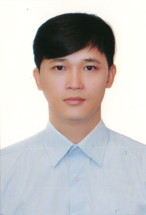
\includegraphics[width=1in,height=1.25in,clip,keepaspectratio]{author/PQV.png}}]{Quang-Vinh Pham}
received the B.Eng. degree in Electronics and Telecommunications in 2012 and the Master’s degree in Data Science in 2024, both from Quy Nhon University, Vietnam. He is currently an AI Engineer at TMA Tech Group, Vietnam. His research interests include Natural Language Processing, Computer Vision, and Physical AI.
\end{IEEEbiography}
\vspace{-15.0cm}
\begin{IEEEbiography}[{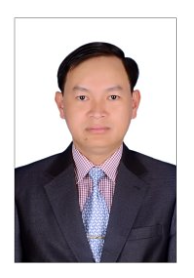
\includegraphics[width=1in,height=1.25in,clip,keepaspectratio]{author/Myteacher.png}}]{Quang-Hung Le}
received the Ph.D. degree in Computer Science from the University of Engineering and Technology, Vietnam National University, Hanoi, in 2016. He is currently a lecturer with the Department of Information Technology, Quy Nhon University, Vietnam. His research interests include Natural Language Processing, Machine Learning, Artificial Intelligence, and Recommender Systems.
\end{IEEEbiography}

\end{document}
